\documentclass[a4paper,12pt]{article}

%%% Работа с русским языком
\usepackage{cmap}					% поиск в PDF
\usepackage{mathtext} 				% русские буквы в формулах
\usepackage[T2A]{fontenc}			% кодировка
\usepackage[utf8]{inputenc}			% кодировка исходного текста
\usepackage[english,russian]{babel}	% локализация и переносы
\usepackage{xcolor}
\usepackage{hyperref}
 % Цвета для гиперссылок
\definecolor{linkcolor}{HTML}{799B03} % цвет ссылок
\definecolor{urlcolor}{HTML}{799B03} % цвет гиперссылок

\hypersetup{pdfstartview=FitH,  linkcolor=linkcolor,urlcolor=urlcolor, colorlinks=true}

%%% Дополнительная работа с математикой
\usepackage{amsfonts,amssymb,amsthm,mathtools} % AMS
\usepackage{amsmath}
\usepackage{icomma} % "Умная" запятая: $0,2$ --- число, $0, 2$ --- перечисление

%% Номера формул
%\mathtoolsset{showonlyrefs=true} % Показывать номера только у тех формул, на которые есть \eqref{} в тексте.

%% Шрифты
\usepackage{euscript}	 % Шрифт Евклид
\usepackage{mathrsfs} % Красивый матшрифт

%% Свои команды
\DeclareMathOperator{\sgn}{\mathop{sgn}}

%% Перенос знаков в формулах (по Львовскому)
\newcommand*{\hm}[1]{#1\nobreak\discretionary{}
{\hbox{$\mathsurround=0pt #1$}}{}}
% графика
\usepackage{graphicx}
\graphicspath{{pictures/}}
\DeclareGraphicsExtensions{.pdf,.png,.jpg}

\usepackage[left=25mm, top=30mm, right=25mm, bottom=30mm, nohead, nofoot]{geometry}

\author{Бурмашев Григорий, БПМИ-208}
\title{Язык SQL, дз -- 8 }
\date{\today}
\begin{document}
\maketitle
\section*{Номер 2}
\begin{center}

\includegraphics[scale=0.4]{t2.png}
\end{center}
Вместо фиксации произвожу откат, код, произведенный в первом терминале:
\begin{center}
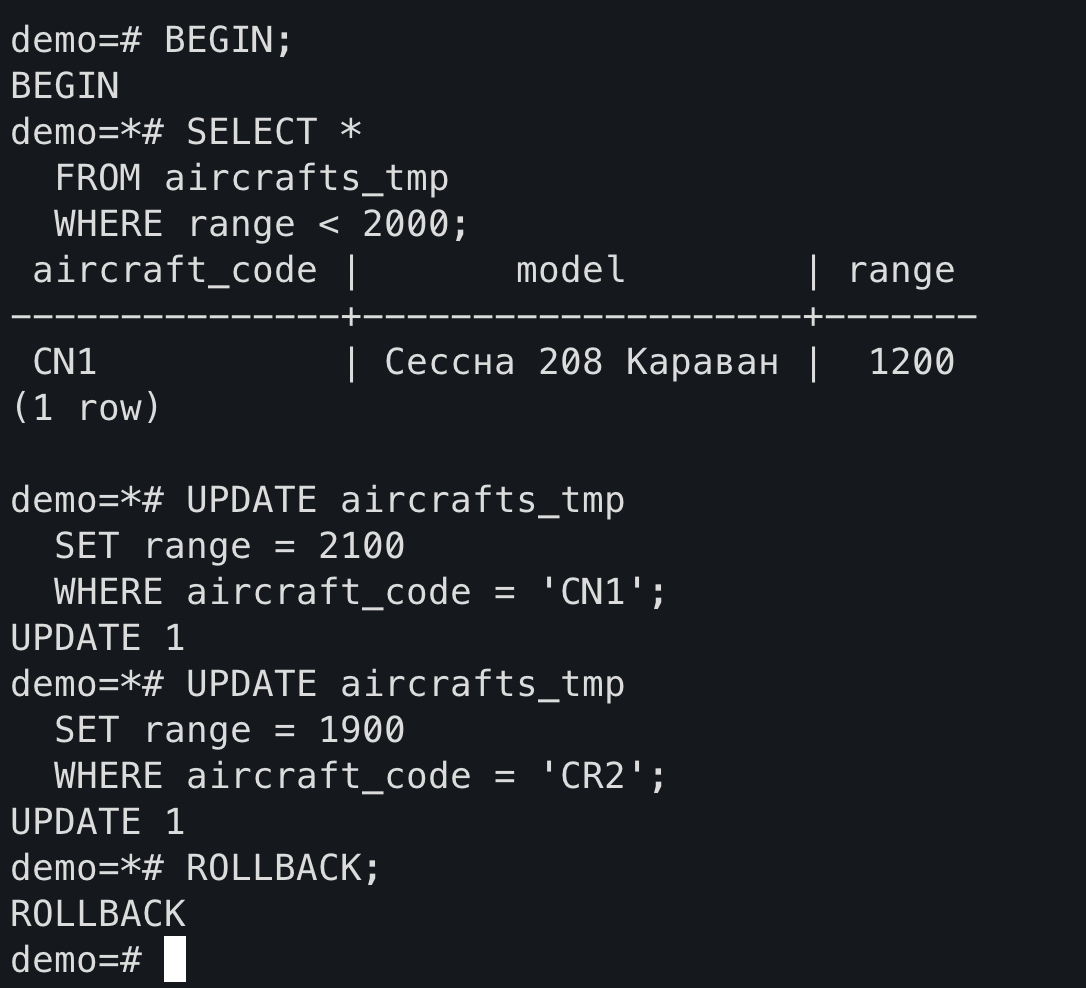
\includegraphics[scale=0.6]{21.png}
\end{center}
Во втором терминале же получили следующий результат:
\begin{center}
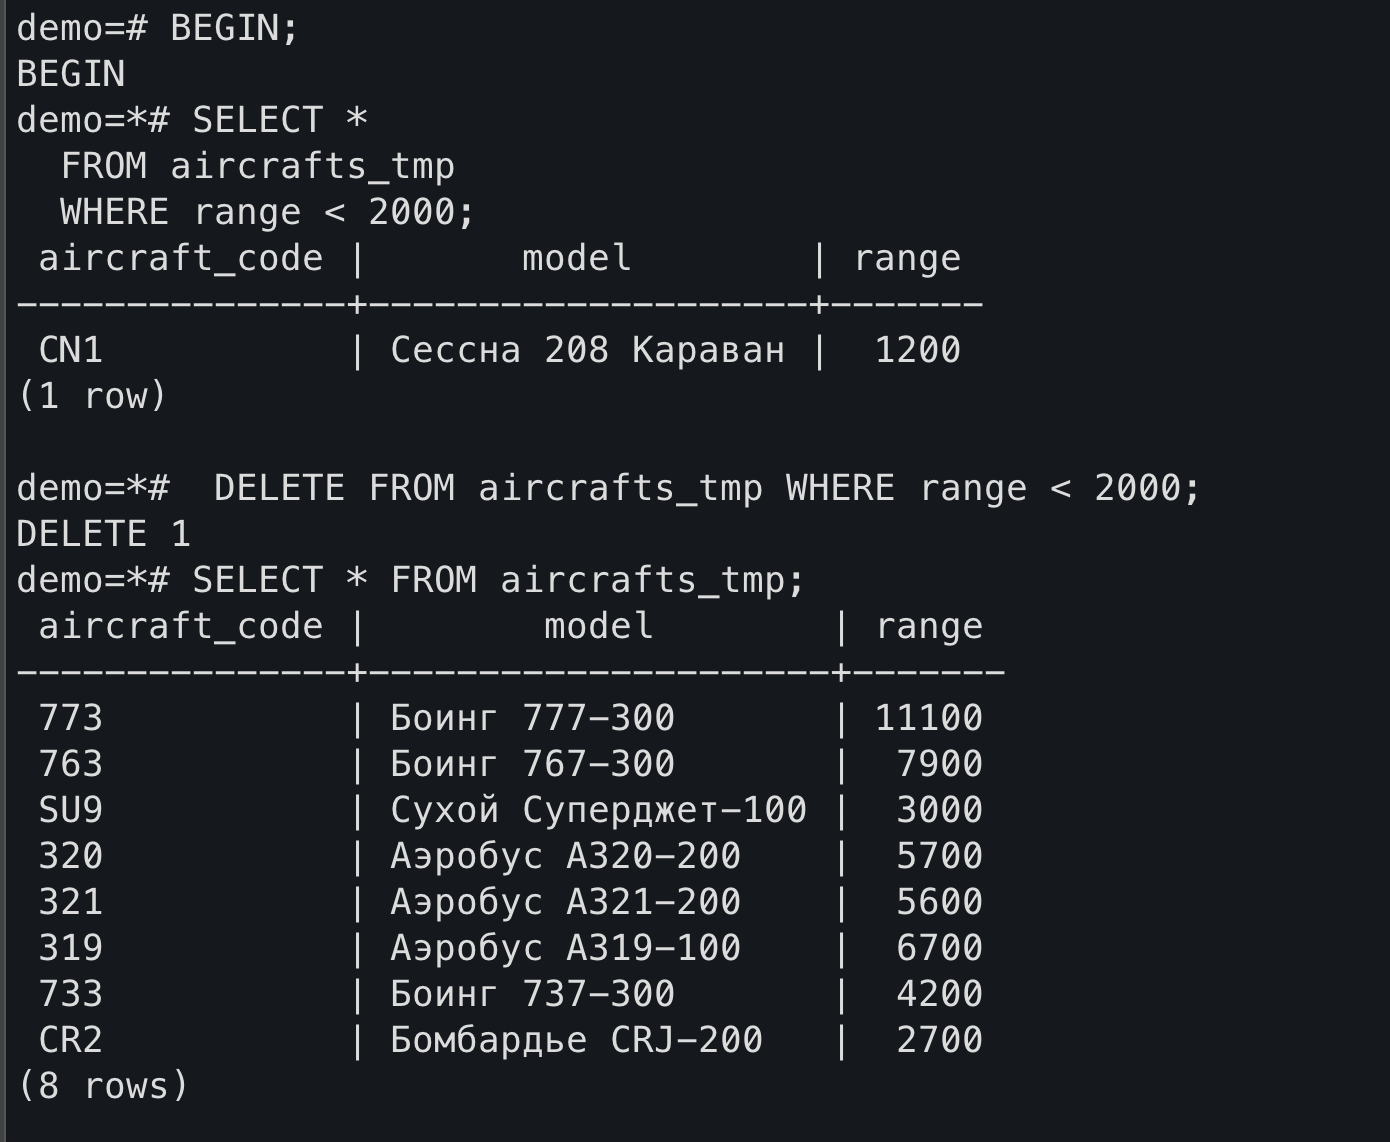
\includegraphics[scale=0.6]{22.png}
\end{center}
Видим, что в результате отката первой транзакции её результаты не сохранились, а следовательно вторая транзакция привела к удалению строки с \textbf{model = Сессна 208 Караван}, поскольку у этого самолета изначальная дистанция (до 1 транзакции) меньше 2000
\clearpage
\section*{Номер 3}
\begin{center}
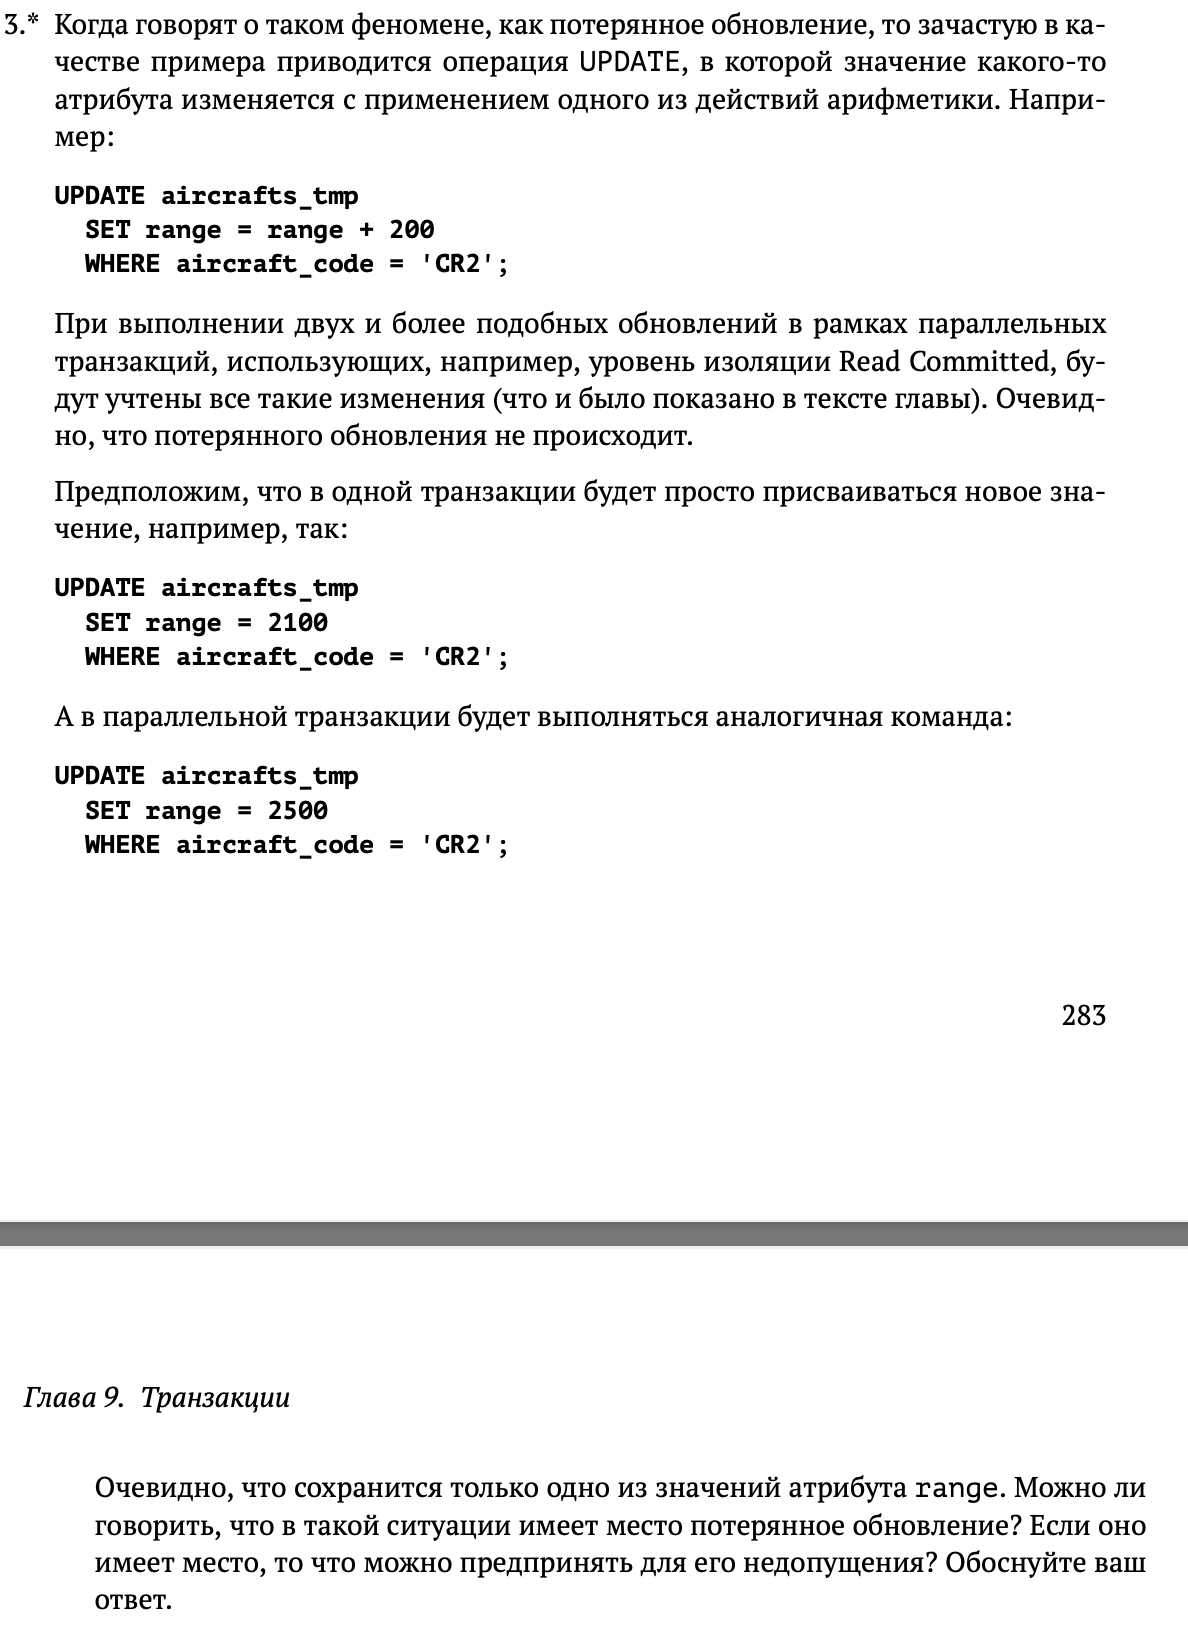
\includegraphics[scale=0.6]{t3.png}
\end{center}
Да, в такой ситуации имеет место потерянное обновление, поскольку одна из двух  транзакций перезапишет данные, которые были обновлены другой транзакцией, вероятно пользователь хочет видеть от базы данных другого поведения (например запрета выполнения таких транзакций одновременно)
\end{document}
